\chapter{Tree Computations}

Consideriamo adesso una serie di problemi computazionali su alberi. Come possiamo osservare, gli alberi hanno una struttura asimmetrica, e questo ci permette di risolvere alcuni problemi in modo più efficiente e semplice rispetto ai grafi generici o a struttura nelle quali è difficile rompere la simmetria. Infatti, non è necessario utilizzare tecniche di rottura della simmetria, come ad esempio l'assegnazione di ID unici ai nodi, per risolvere problemi su alberi.

Infatti, un nodo all'interno di albero può identificare la propria posizione all'interno della struttura,
\begin{itemize}
    \item Un nodo sa di essere una \textit{foglia} in quanto ha grado 1 ($N(x) = 1$), mentre è un nodo \textit{interno} se ha grado maggiore di 1 ($N(x) > 1$).
        \item Un altra proprietà importante è che ogni tipologia di albero ha almeno due foglie.
        \usetikzlibrary{chains}
        \begin{center}
            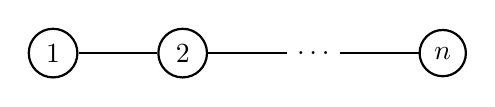
\begin{tikzpicture}[start chain=going right, node distance=10mm, every node/.style={on chain, join}, thick]
                \node[circle,draw] {1};
                \node[circle,draw] {2};
                \node[draw=none] {$\dots$};
                \node[circle,draw] {$n$};
            \end{tikzpicture}
        \end{center}
\end{itemize}

Introduciamo la tecnica di \textit{saturazione}, che ci permette di risolvere problemi su alberi in ambiente distribuito in modo efficiente.

\section{Saturation Technique}

Consideriamo un ambiente distribuito con una topologia ad albero e sia tale informazione, riguardante la struttura topologica, nota a tutti i nodi della rete. La tecnica di saturazione consiste nell'identifacare una singola coppia di nodi adiacenti all'interno della rete. Tale coppia di nodi sarà in grado di far iniziare altre computazioni. In pratica, la tecnica di saturazione consiste nell'eleggere un arco della rete. Osserviamo che non c'è nessuna garanzia su quale arco venga eletto: questa tecnica garantisce l'elezione di uno fra i possibili archi, ma non garantisce quale arco venga eletto.

Tipicamente la tecnica di saturazione è usata per risolvere problemi distribuiti di varia natura. In particolare, la saturazione è inserita all'interno di un processo più grande, che può essere diviso nelle seguenti tre fasi:
\begin{itemize}
    \item \textbf{Attivazione}: in questa fase, i nodi iniziatori attivano i restanti nodi della rete utilizzando un protocollo di \texttt{wake-up}.
    \item \textbf{Saturazione}: in questa fase, a partire dalle foglie si identifica un'unica coppia di nodi adiacenti, anche detti \textit{nodi saturati}.
    \item \textbf{Risoluzione}: in questa fase, i nodi saturati danno inizio ad una o più computazioni necessarie alla risoluzione di uno specifico problema distribuito.
\end{itemize}

Ci focalizziamo ora a definire le prime due fasi poiché la terza fase dipende dal problema specifico che si vuole risolvere. Definiamo la tripla $\langle P_{init}, P_{final}, R\rangle$ e sia $T = (V, E)$ l'albero considerato. Sia inoltre $W \subseteq V,\ W \neq \empty$ l'insieme dei nodi \texttt{initiator}. Allora
\begin{itemize}
    \item $P_{init}$: $\forall x \in V:$, 
    \[
        status(x) = \begin{cases*}
            \texttt{awake} & se $x \in W$\\
            \texttt{asleep} & altrimenti
        \end{cases*}
    \]
    \item $P_{final}$: $\exists! (u, v) \in E: status(u) = status(v) = \texttt{saturated}$ e $\forall w \in V\setminus\{u, v\}: status(w) = \texttt{active}$, ossia tutti i nodi tranne $u$ e $v$ sono attivi, mentre $u$ e $v$ sono saturati.
    \item $R = \{\texttt{TR, BL, CN, KT, MO}\}$, dove \\ \texttt{KT = Knowledge of the Topology} e \texttt{MO = Message Ordering}.
\end{itemize}

Siano
\begin{itemize}
    \item $S = \{\texttt{available, active, processing, saturated}\}$ l'insieme degli stati dei nodi,
    \item $S_{init} = \{available\}$ l'insieme degli stati iniziali dei nodi,
    \item $S_{final} = \{active, saturated\}$ l'insieme degli stati finali dei nodi.
\end{itemize}

\section{Minimum Finding}

\section{Eccentricities \& Center Finding}